\documentclass{beamer}
\usetheme{metropolis}           % Use metropolis theme
\title{\LaTeX \  und Marxismus}
\usepackage{breqn}
\date{\today}
\author{Kimi Müller}
% \institute{Centre for Modern Beamer Themes}
\begin{document}
  \maketitle
  \section{WZF?!}
  \begin{frame}{Zwei Themen?}
    \begin{itemize}
        \item<1-> \textbf{Problem:} Ich möchte gerne über Marxismus reden, habe aber viel Aufwand in die Präsentation gesteckt.
        \item<2-> \textbf{Lösung:} Ich referiere kurz über \LaTeX und danach über Marxismus.
        \item<3-> \textbf{Grundlage:} Thema ist frei wählbar
    \end{itemize}
  \end{frame}
  \begin{frame}
    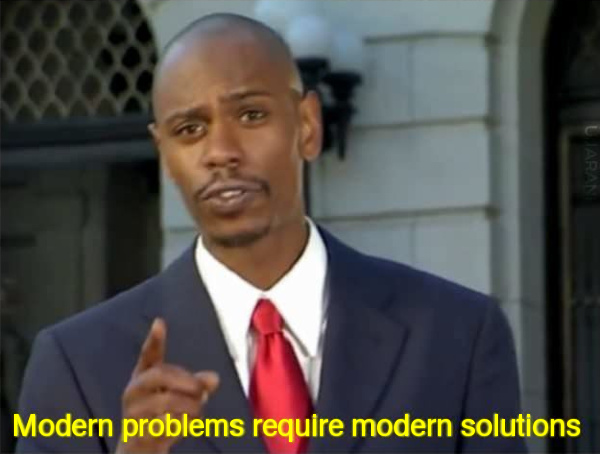
\includegraphics[width=\textwidth]{Modern_Problems_Require_Modern_Solutions.jpg}
  \end{frame}
  \begin{frame}{Agenda}
\begin{itemize}
    \item<2-> Disclaimer
    \item<3-> Was ist \LaTeX?
    \item<4-> Warum \LaTeX?
    \item<5-> Was ist Kommunismus?
    \item<6-> Warum Kommunismus?
    \item<7-> Mehrwerttheorie
    \item<8-> Stummer Zwang der materiellen Verhältnisse
    \item<9-> Reservearmee des Kapitals
\end{itemize}
  \end{frame}
  \begin{frame}{Disclaimer}
\textbf{Ich bin kein Experte in \LaTeX, Kommunismus oder Präsentationen. Ich liebe die Freiheitlich-Demokratische Rechtsordnung, diese Präsentation dient nur zu theoretischen und Unterhaltungszwecken.}
\end{frame}
  \section{Was ist \LaTeX?}
  \begin{frame}{WYSIWYG}
    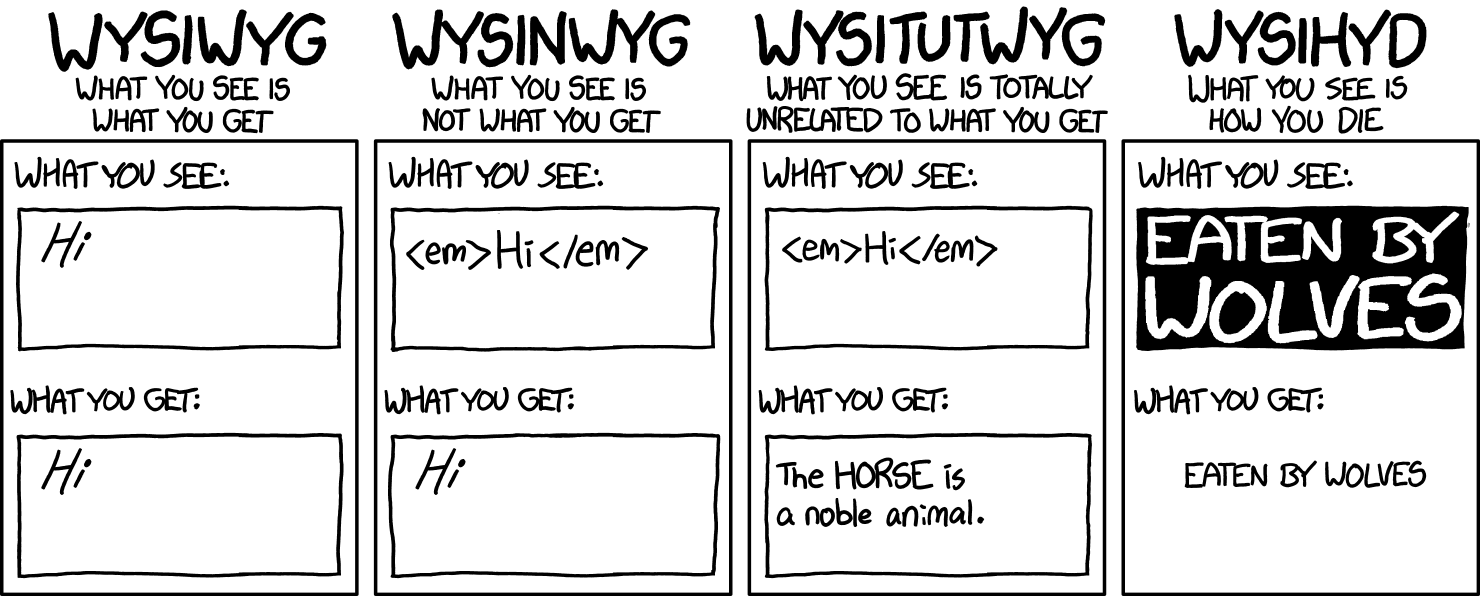
\includegraphics[width=\textwidth]{types_of_editors_2x.png}
  \end{frame}
  \begin{frame}{Echtes Beispiel dieser Präsentation}
  \end{frame}
  \section{Warum \LaTeX?}
  \begin{frame}
\begin{dmath}
  Q(\lambda,\hat{\lambda}) = -\frac{1}{2} P{(O \mid \lambda )} \sum_s \sum_m \sum_t \gamma_m^{(s)} (t) \left( n \log(2 \pi ) + \log \left| C_m^{(s)} \right| + \left( \mathbf{o}_t - \hat{\mu}_m^{(s)} \right) ^T C_m^{(s)-1} \left(\mathbf{o}_t - \hat{\mu}_m^{(s)}\right) \right)
\end{dmath}
\end{frame}
\begin{frame}{Dasselbe in Word}
\href{https://i.makeagif.com/media/5-28-2022/dXcfrH.gif}{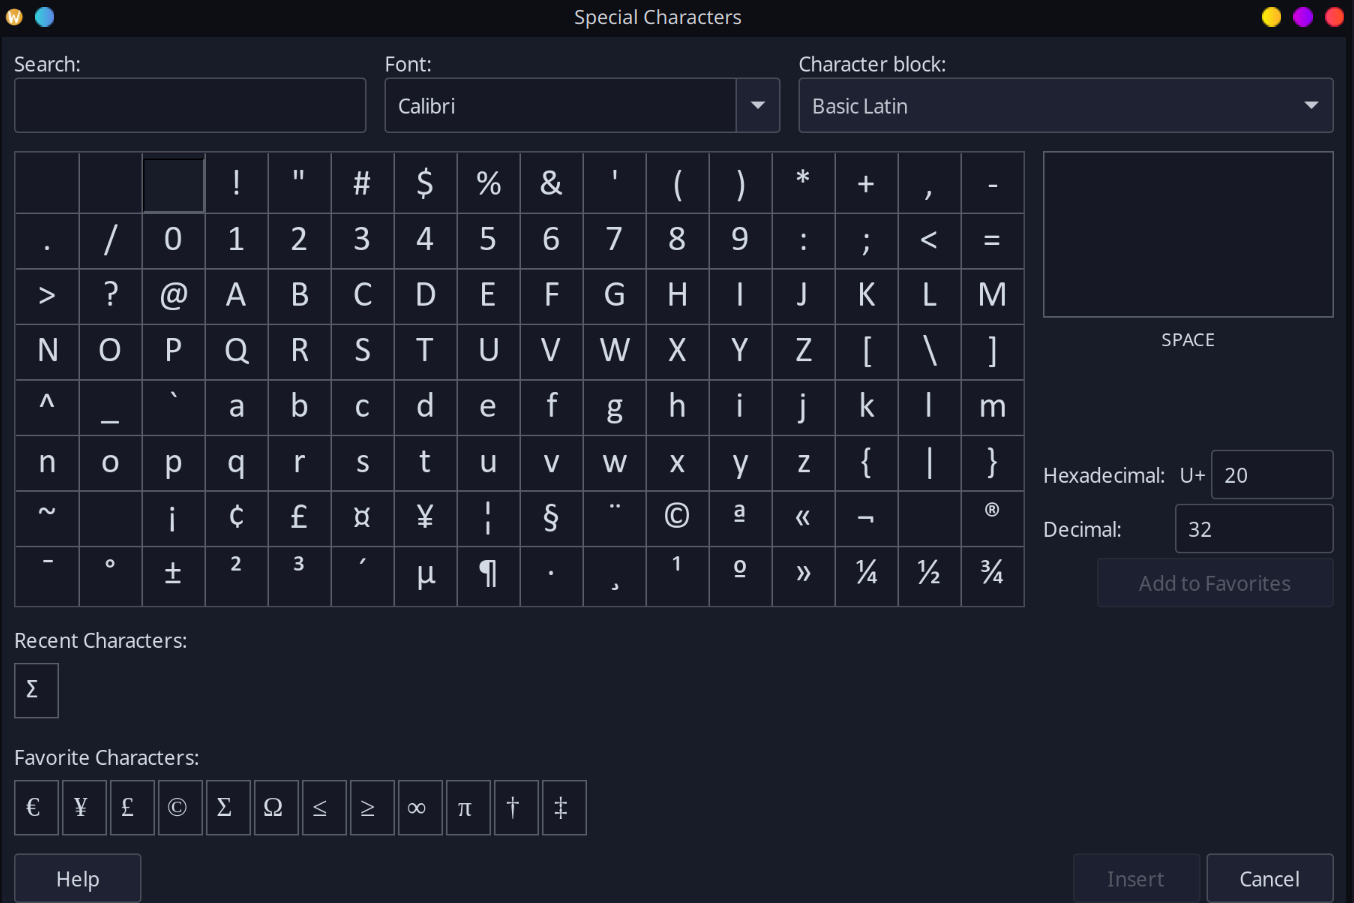
\includegraphics[width=\textwidth]{FormelnWord.png}}
\end{frame}
\begin{frame}
\href{Link mit einsteigerfreundlichen Informationen}{https://www.overleaf.com/}
\end{frame}

\begin{frame}{Eigenschaften von \LaTeX}
    \begin{itemize}
        \item<2-> Beitrag von Vielen für Viele
        \item<3-> Große Community
        \item<4-> Komplexe Anwendung, aber simples Konzept
        \item<5-> Funktioniert besser als man denkt
        \item<6-> Belächelt von Menschen, die es nicht verstehen
    \end{itemize}

        $\Rightarrow$ auf den ersten Blick unattraktiv, aber unterschätzt.
\end{frame}

\begin{frame}{Eigenschaften von \LaTeX\ und Kommunismus}
    \begin{itemize}
        \item Beitrag von Vielen für Viele
        \item Große Community
        \item Komplexe Anwendung, aber simples Konzept
        \item Funktioniert besser als man denkt
        \item Belächelt von Menschen, die es nicht verstehen
    \end{itemize}
        $\Rightarrow$ auf den ersten Blick unattraktiv, aber unterschätzt.
\end{frame}
\begin{frame}{Mehrwerttheorie}

\end{frame}
\end{document}
